\chapter{Heterogeneity in the MAX phases}

\graphicspath{{Chapter3/Figs/}}


As  discussed in \autoref{sec:ductility_criteria} the MAX phases are predicted to be brittle by a wide range of ductility criteria but they are in fact observed to be damage tolerant and to flow easily in the basal plane \cite{Barsoum1999}.
Predictions of the Peierls stress made using the methods described in \autoref{sec:dislocations} have been made previously \cite{Music2007ductility,Gouriet2015}, however these have had limited success, producing over estimates, for example \citet{Gouriet2015} reported the Peierls stress to be at least \SI{611}{\mega\pascal} which is in fact slightly higher than that estimated for titanium carbide and other very hard brittle materials in which slip is limited at room temperature by the Peierls mechanism \cite{Chang1966,Clegg2006,Kamimura2011,Yadav2014}. Given that flow stresses in the region of a few tens of \si{\mega\pascal} have been observed at room temperature \cite{Humphrey2012,Barsoum1999}, which is more comparable with FCC metals than FCC carbides, it is reasonable to expect the Peierls stress to be lower than this.

The poor performance of Peierls models for MAX phases, and potentially for other complex phases, is possibly due to the treatment of the MAX phase unit cell as homogeneous elastically. This is surprising because many studies have discussed the heterogeneity of the bonding and electron structure, a recent review was written by \citet{Magnuson2017}, and discusses the complex and mixed nature of the bonding varying across the different atomic sites, more metallic in the MA layers, more covalent in the MX layers, and charge transfer contributing an ionic component to the bonding. Clearly this bonding is necessary for many of the MAX phases intriguing properties, e.g. high melting point, high specific stiffness, electrical and thermal conductivity, and a near zero Seebeck coefficient to name a few \cite{Yoo2000,Sun2011,Magnuson2017} but the clear and strong heterogeneity of the unit cell has largely been neglected when considering the dislocation properties of the MAX phases, the only account made for it being the choice of plane at which the generalised stacking fault energy was calculated.

If the MAX phases are elastically heterogeneous there is the uestion of what might be the expected properties and where within the MAX phase unit cell. A simple metric to characterise the chemical heterogeneity is the electronegativity, $\chi$, of regions within the unit cell. For both the M--X and M--A regions, an average electronegativity is easily calculated as once sharing of atoms between the regions is accounted for there are equal numbers of M and A atoms in the M--A region and similarly equal numbers of M and X atoms in the M--X region. The difference in electronegativity between the two regions is therefore defined by
\begin{equation}
\Delta \chi = \frac{\chi_{\text{X}} - \chi_{\text{A}}}{2}
\end{equation}
since the M atoms contribute to both regions. There are a variety of measures of electronegativity, but perhaps the most fundamental is the Mulliken scale \cite{Mulliken1934}, which takes the electronegativity of a species to be the average of the ionization energy, the energy change on removing an electron, and the electron affinity, the energy change on adding an electron. This scale is more fundamental than others because it is calculated from the fundamental properties of atoms, as opposed to more ``relative'' scales that are calculated from enthalpies of formation and covalent radii and so on \cite{huheey1983ch3_electronegativity}.

Since the elements that take the X site, carbon and nitrogen, are generally more electronegative than those that take the A site, elements like aluminium and silicon, it is expected that electron transfer into the M--X region from the M--A. Such a transfer would be expected to increase the strength of the bonding in the M--X layer and reduce it in the M--A, with a corresponding change in the modulus.

\section{Calculating the local stiffness}

Measuring single crystal elastic constants for the MAX phases is extremely difficult due to the difficulty of growing single crystals and experimentally determining the stiffness of sub-unit cell regions of the crystal presents an even greater challenge. Instead density functional theory can be employed. DFT has been widely used to calculate single crystal elastic constants of a large variety of materials and is considered reliable and reproducible \cite{Lejaeghere2016}. One commonly used method for calculating the elastic constants via DFT is simply to simulate the unit cell with periodic boundary conditions and apply a stress/strain state and fit either the equation
\begin{equation}
\sigma_{ij} = C_{ijkl} \epsilon_{kl}
\end{equation}
or 
\begin{equation}
u = \frac{1}{2} C_{ijkl} \epsilon_{ij} \epsilon_{kl}
\end{equation}
where $\sigma_{ij}$ is the stress tensor, $\epsilon_{ij}$ is the strain tensor, $u$ is the strain energy per unit volume and $C_{ijkl}$ is the stiffness tensor. This was applied by \citet{Aryal2014} to a very wide range of MAX phases. Care must be taken to reproduce the physically realistic situation where the stress is equal throughout the unit cell but the strain can vary, that is the strain must be applied macroscopically (i.e. to the simulation cell) but the atomic positions must be allowed to vary to find the lowest energy configuration.

The latter equation was used to find the local stiffness within a region of the unit cell. The single crystal elastic constants must be dropped since a tensor formulation of heterogeneous elasticity is not the aim, instead local shear moduli are calculated. The unit cell is divided naturally into two distinct regions that are obvious from the geometry of the crystal structure, the local chemistry and nature of bonding, there is a more metallic layer, the M--A layer, and a more covalent layer, the M--X layer, see \label{fig:fig:MAX_unit_cells}. The layer of M-atoms that are bonded to both A-atoms and X-atoms is the natural boundary.

To localise the strain in, say, the M--A layer all the bonding, that is the relative atomic positions, in the M--X layer are held rigid and are displaced as a whole such that in each M--A layer the appropriate strain is applied. The relative positions of the atoms within the M--A layer are then allowed to relax to achieve the minimum energy. The equation that must then be fitted is
\begin{equation}
u = \frac{1}{2} G_{i} \gamma^2
\end{equation}
where $\gamma$ is the applied strain and $G_i$ is the local shear modulus, namely either $G_{M\text{--}A}$ or $G_{M\text{--}X}$. The procedure is applied vice versa to calculate the M--X properties.




\begin{figure}
\centering
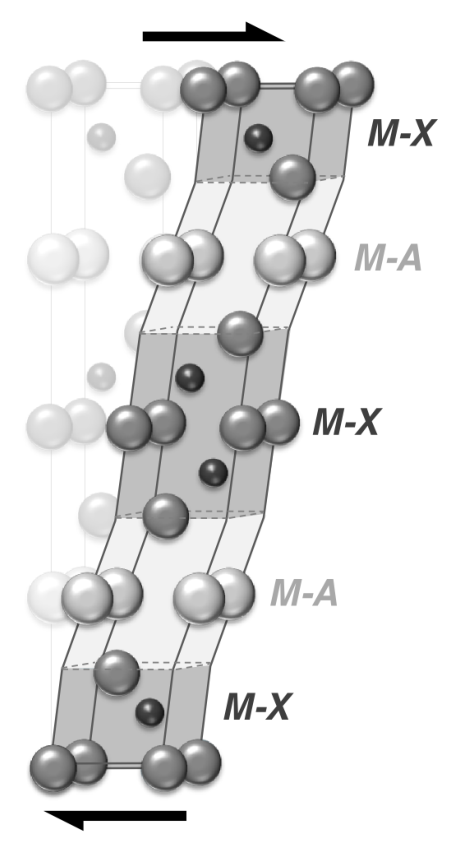
\includegraphics[height=0.3\textheight]{slab_model}
\caption{Schematic of non-uniform elastic deformation in a ``211'' MAX phase showing the regions that might be considered distinct, the M--A and M--X layers.}
\end{figure}



The overall shear modulus for the whole crystal structure is calculated in the same manner with no restrictions on the atomic positions, all the atoms are allowed to relax fully. Since this relaxed shear is equivalent to a uniform applied stress an analogy is possible with the assumptions made to calculate the transverse stiffness of long fibre composite materials, the so called slab model \cite{Hull1996ch4}. The slab model is illustrated in . The results of the local calculations can be compared with the overall case using the equation:

\begin{equation}
G_{\text{slab}} = \left[ \frac{f_{M\text{--}X}}{G_{M\text{--}X}} + \frac{f_{M\text{--}A}}{G_{M\text{--}A}} \right]^{-1}
\end{equation}
where $G_{\text{slab}}$ is the estimate for the overall shear modulus, $f_i$ is the volume fraction of the region $i$ and $G_i$ is the shear modulus of region $i$. The volume fractions are estimated from the crystal structures of the MAX phases. In particular the fractional coordinate in the $c$ direction of the M1 site in the ``211'' phases, $z_1$, and the position of the M2 site in the ``312'' and ``413'' phases, $z_2$, as shown in \autoref{fig:MAX_unit_cells}, determines the volume fraction of the regions of the unit cell.












